% Requirements are LaTeX (e.g. texlive), TikZ, and rubber.
% Build using the following command.
% rubber --pdf full-description


\documentclass{article}

\usepackage{subfig}
\usepackage{tikz}
\usetikzlibrary{arrows,positioning}

\begin{document}


% This rate matrix figure copypasted from ratematrix.tex.
\begin{figure}
\centering
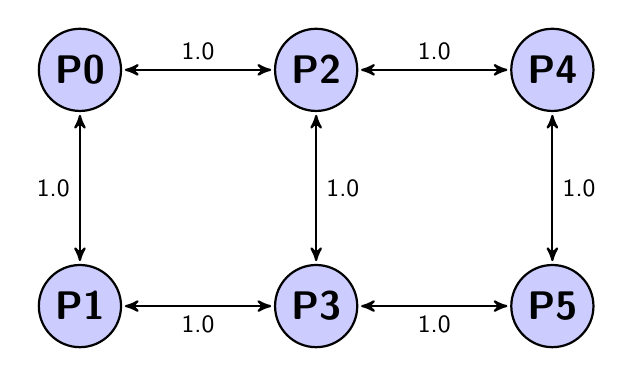
\begin{tikzpicture}[<->,>=stealth',shorten >=1pt,shorten <=1pt,
  auto,node distance=3cm,thick,
  main node/.style={circle,fill=blue!20,draw,font=\sffamily\Large\bfseries}]

  \node[main node] (0) {P0};
  \node[main node] (1) [below of=0] {P1};
  \node[main node] (2) [right of=0] {P2};
  \node[main node] (3) [below of=2] {P3};
  \node[main node] (4) [right of=2] {P4};
  \node[main node] (5) [below of=4] {P5};

  \path[every node/.style={font=\sffamily\small}]
    (0) edge node [left] {1.0} (1)
    (2) edge node [right] {1.0} (3)
    (4) edge node [right] {1.0} (5)
    (0) edge node [above] {1.0} (2)
    (2) edge node [above] {1.0} (4)
    (1) edge node [below] {1.0} (3)
    (3) edge node [below] {1.0} (5);

\end{tikzpicture}
\caption{
	The neutral unscaled substitution rates
	among the primary (codon-like) states
	P0, P1, P2, P3, P4, and P5.
}
\end{figure}

% This simplified codon model figure is from code.tex.
\begin{figure}
\centering
\begin{tabular}{c c}
  primary & tolerance \\
  state & class \\
  \hline
  P0 & T0 \\
  P1 & T0 \\
  P2 & T1 \\
  P3 & T1 \\
  P4 & T2 \\
  P5 & T2
\end{tabular}
\caption{
	Each primary state is associated with a tolerance class.
	Tolerance classes are like amino acids,
	and primary states are like codons.
	Therefore this table is like a toy genetic code.
}
\end{figure}

% This tree figure is from tree.tex.
\begin{figure}
\centering
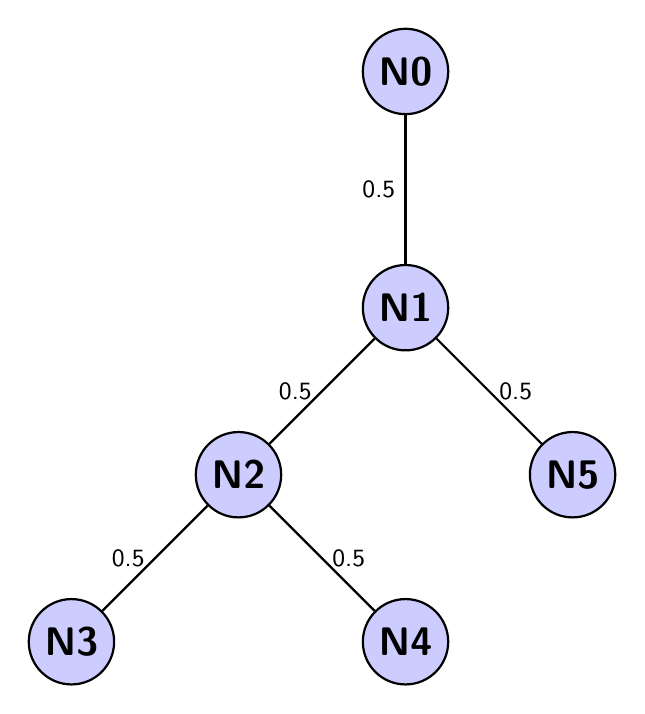
\begin{tikzpicture}[-,>=stealth',auto,node distance=3cm,thick,
  main node/.style={circle,fill=blue!20,draw,font=\sffamily\Large\bfseries}]

  \node[main node] (0) {N0};
  \node[main node] (1) [below of=0] {N1};
  \node[main node] (2) [below left of=1] {N2};
  \node[main node] (3) [below left of=2] {N3};
  \node[main node] (4) [below right of=2] {N4};
  \node[main node] (5) [below right of=1] {N5};

  \path[every node/.style={font=\sffamily\small}]
    (0) edge node [left] {0.5} (1)
    (1) edge node [left] {0.5} (2)
    (2) edge node [left] {0.5} (3)
    (2) edge node [right] {0.5} (4)
    (1) edge node [right] {0.5} (5);

\end{tikzpicture}
\caption{
	This tree will be used for the toy example.
	The branch lengths define the expected number of
	primary state transitions (analogous to codon substitutions)
	when the primary process is unconstrained by selection.
	In general, fewer primary state transitions would be expected
	when selection is at work, for example in the reference process
	(as opposed to the default process) in the irreversible-switch model,
	or when some tolerance classes are in the untolerated state
	in the blinking model.
}
\end{figure}

% This figure merges two figures from data.tex.
\begin{figure}
\centering
\begin{tabular}{c c c c c}
	     & primary &    &    &    \\
	node & state   & T0 & T1 & T2 \\
  \hline
  N0 & P0 & on & (off) & (on) \\
  N1 & ? & ? & ? & ? \\
  N2 & ? & ? & ? & ? \\
  N3 & P4 & ? & ? & on \\
  N4 & P5 & ? & ? & on \\
  N5 & P1 & on & ? & ?
\end{tabular}
\caption{
	This table provides primary state and tolerance state data.
	Some of the nodes have known primary states.
	This is analogous to alignment data for a single codon site.
	For some of the nodes,
	some of the tolerance classes have known states.
	The states enclosed by parentheses represent
	disease data.
}
\end{figure}



\end{document}




